\section{Analyses}
\label{sec:analysis}

We conduct in-depth analyses to understand where the advantage of GraphPTC comes from and how the execution graph changes tool-calling behavior.

\begin{figure}[t]
\centering
\begin{subfigure}{0.32\linewidth}\centering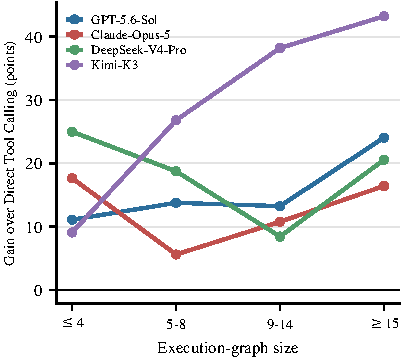
\includegraphics[width=\linewidth]{figs/scaling.pdf}\caption{Gain by execution-graph size}\label{fig:scaling}\end{subfigure}\hfill
\begin{subfigure}{0.32\linewidth}\centering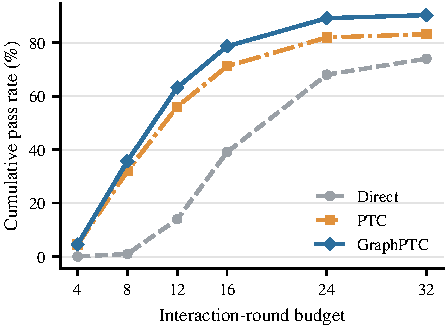
\includegraphics[width=\linewidth]{figs/efficiency.pdf}\caption{Accuracy vs. round budget}\label{fig:efficiency}\end{subfigure}\hfill
\begin{subfigure}{0.32\linewidth}\centering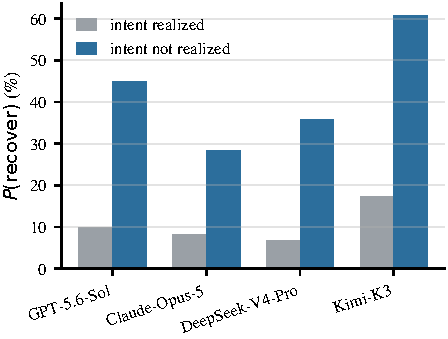
\includegraphics[width=\linewidth]{figs/recovery.pdf}\caption{Recovery probability by intent}\label{fig:recovery}\end{subfigure}
\caption{Analyses of GraphPTC on AppWorld, averaged over four backbones. (\subref{fig:scaling}) The gain over Direct Tool Calling is positive in every complexity bin, and its average widens toward the most complex tasks. (\subref{fig:efficiency}) Along the accuracy against interaction-round frontier GraphPTC reaches the accuracy of Direct Tool Calling with fewer rounds. (\subref{fig:recovery}) An intent that is not realized raises the probability that the agent issues a recovery action.}
\label{fig:analysis}
\end{figure}

\subsection{Ablation Study on Graph Modeling}

To locate the contribution of the graph layer, we ablate the two structural changes and report the five-backbone average of each setting.
Removing the execution graph and its graph-guided recovery reduces GraphPTC to PTC, where a block reports a plain success flag with raw output instead of typed effects, and removing the programmatic runtime as well reduces it to Direct Tool Calling.
As shown in Table~\ref{tab:ablation}, the execution graph is worth $6.3$ points on average and stays positive on all seven settings, while the programmatic runtime by itself is worth only $0.5$ points and turns negative on four of them, so writing code by itself does not reliably improve on Direct Tool Calling and the graph is what turns it into a consistent gain.

The size of the graph contribution tracks how much cross-block dependency a setting carries, reaching $11.7$ points on BrowseComp-Plus and $8.3$ points on AppWorld-Normal, where a result produced in one block is consumed by a later block, and falling to $1.9$ points on FRAMES, where most questions resolve within a few independent lookups.
The loss of plain PTC concentrates in the same settings and on one backbone, since its worst cells are $-33.0$ points on BrowseComp-Plus and $-34.5$ points on AppWorld-Normal, both on Claude-Opus-5, which loses $10.5$ points under plain PTC while the other four backbones gain from it.

\begin{table}[t]
\centering\scriptsize
\setlength{\abovecaptionskip}{0pt}
\setlength{\belowcaptionskip}{0pt}
\setlength{\tabcolsep}{4pt}
\newcommand{\hdc}[2]{\begin{tabular}[b]{@{}c@{}}\textbf{#1}\\\textbf{#2}\end{tabular}}
\caption{Ablation of the two structural changes of GraphPTC, reported per setting as the five-backbone average. PTC removes the execution graph and Direct Tool Calling removes the programmatic runtime as well, and the last two rows split the total gap into the contribution of each change.}
\label{tab:ablation}
\resizebox{\linewidth}{!}{%
\begin{tabular}{l ccccccc c}
\toprule
\textbf{Configuration}
 & \hdc{BrowseComp-}{Plus} & \hdc{AppWorld-}{Normal} & \hdc{AppWorld-}{Challenge} & \textbf{Agent-Diff} & \textbf{FanOutQA} & \textbf{FRAMES} & \hdc{Automation-}{Bench} & \textbf{Avg} \\
\midrule
\textbf{GraphPTC} (full)              & \best{39.1} & \best{92.1} & \best{88.4} & \best{72.7} & \best{63.7} & \best{81.0} & \best{31.7} & \best{67.0} \\
\;\; $-$ execution graph              & 27.4 & 83.8 & 83.7 & 67.3 & 55.2 & 79.1 & 27.8 & 60.6 \\
\;\; $-$ execution graph and programs & 33.1 & 82.4 & 69.3 & 69.7 & 61.2 & 79.4 & 26.0 & 60.2 \\
\midrule
Contribution of the execution graph     & $+11.7$ & $+8.3$ & $+4.7$ & $+5.4$ & $+8.5$ & $+1.9$ & $+3.9$ & $+6.3$ \\
Contribution of the programmatic runtime & $-5.7$ & $+1.4$ & $+14.4$ & $-2.4$ & $-6.0$ & $-0.4$ & $+1.8$ & $+0.5$ \\
\bottomrule
\end{tabular}%
}
\end{table}

\subsection{Advantage of Non-Linear Recovery}

To test whether modeling cross-block dependency as a graph enables recovery a linear history cannot, we study how the agent uses the actions that return to a specific node.
We measure the probability that the agent issues a recovery action conditioned on whether the previous block realized its declared intent, and on the tasks where GraphPTC uses recovery we compare its pass rate with PTC on the same task identifiers.
As shown in Figure~\ref{fig:recovery}, an unrealized intent raises the recovery probability by three to five times across backbones, so the declared-and-verified intent is an actionable signal that the agent responds to.
On the same task identifiers GraphPTC exceeds PTC, and since the comparison fixes the task and differs mainly in whether the agent can return to a failed node, we read the gap as largely driven by non-linear recovery.

\subsection{Advantage on Complex Long-Horizon Tasks}

To locate where the advantage of GraphPTC arises, we bin every AppWorld task by the number of program blocks in its execution graph and measure the gain of GraphPTC over Direct Tool Calling within each bin.
As shown in Figure~\ref{fig:scaling}, the gain is positive in every bin for every backbone, and its four-backbone average rises from $15.7$ points in the smallest bin to $26.1$ points in the largest.
The widening is carried by GPT-5.6-Sol and Kimi-K3, which reach $24.1$ and $43.2$ points in the largest bin, while Claude-Opus-5 and DeepSeek-V4-Pro gain in every bin without a monotone trend.
A larger task graph holds more intermediate results and more failure-prone steps, so addressable artifacts and local recovery matter more as a linear history grows harder to reconstruct.

\subsection{Efficiency and Token Economy}

To check whether the graph improves efficiency and not only accuracy, we measure the interaction rounds each method spends and trace the accuracy it reaches under a round budget.
On AutomationBench, GraphPTC spends $54$ to $64\%$ fewer model rounds than Direct Tool Calling while raising the pass rate, because one block carries several dependent calls whose intermediate values are registered as artifacts and reused (Appendix~\ref{app:analyses}).
As shown in Figure~\ref{fig:efficiency}, on AppWorld the same effect appears along the accuracy against round frontier, where GraphPTC reaches the accuracy of Direct Tool Calling with about $2$ times fewer rounds and stays on or above the PTC frontier at every budget.
The graph stays in the runtime and enters the model only through the bounded feedback, so the input per round is independent of graph size and the round savings are not offset by a growing context.
As shown in Table~\ref{tab:cost}, GraphPTC reaches higher accuracy than Direct Tool Calling on every benchmark while reading $1.7$ to $2.3$ times fewer input tokens, and uses fewer rounds on all but one benchmark, since a per-call transcript re-sends the growing history on each turn.

\begin{table}[t]
\centering\scriptsize
\setlength{\abovecaptionskip}{0pt}
\setlength{\belowcaptionskip}{0pt}
\setlength{\tabcolsep}{5pt}
\caption{Cost comparison of GraphPTC and Direct Tool Calling, averaged over four backbones. GraphPTC reaches higher accuracy while reading fewer input tokens on every benchmark and using fewer interaction rounds on all but one. \textbf{Bold} marks the better method per metric and benchmark.}
\label{tab:cost}
\resizebox{\linewidth}{!}{%
\begin{tabular}{l cc cc cc}
\toprule
 & \multicolumn{2}{c}{\textbf{Accuracy (\%)}} & \multicolumn{2}{c}{\textbf{Input tokens (k)}} & \multicolumn{2}{c}{\textbf{Rounds}} \\
\cmidrule(lr){2-3}\cmidrule(lr){4-5}\cmidrule(lr){6-7}
\textbf{Benchmark} & Direct Tool Calling & GraphPTC & Direct Tool Calling & GraphPTC & Direct Tool Calling & GraphPTC \\
\midrule
AppWorld-Normal    & 82.3 & \best{90.9} & 151.4 & \best{84.1}  & 16.4 & \best{9.1} \\
AppWorld-Challenge & 68.7 & \best{88.6} & 228.8 & \best{133.5} & 18.7 & \best{11.7} \\
Agent-Diff         & 68.5 & \best{70.8} & 113.2 & \best{49.0}  & 9.6  & \best{6.6} \\
FanOutQA           & 60.0 & \best{62.9} & 128.5 & \best{63.9}  & 8.7  & \best{6.9} \\
FRAMES             & 79.3 & \best{80.6} & 93.0  & \best{55.2}  & \best{5.6}  & 7.1 \\
AutomationBench    & 24.6 & \best{29.0} & 324.4 & \best{171.9} & 36.1 & \best{14.3} \\
\bottomrule
\end{tabular}%
}
\end{table}

\begin{figure}[t]
\centering
\begin{subfigure}{0.32\linewidth}\centering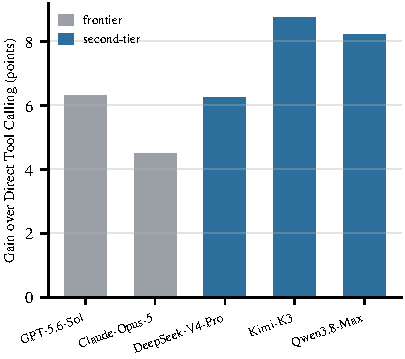
\includegraphics[width=\linewidth]{figs/gain.pdf}\caption{Gain over Direct by backbone}\label{fig:capgain}\end{subfigure}\hfill
\begin{subfigure}{0.32\linewidth}\centering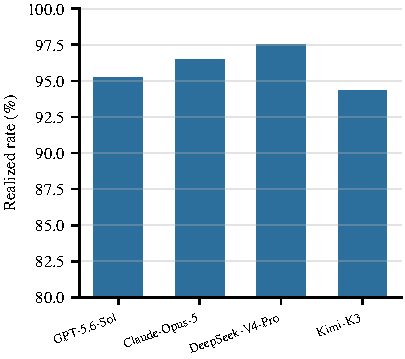
\includegraphics[width=\linewidth]{figs/fidelity.pdf}\caption{Realization rate of intents}\label{fig:fidelity}\end{subfigure}\hfill
\begin{subfigure}{0.32\linewidth}\centering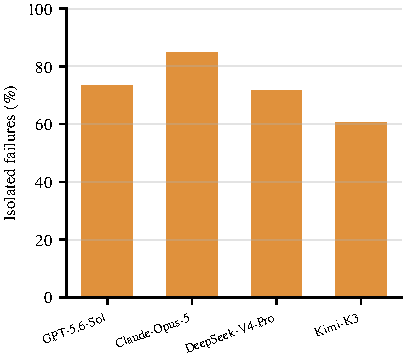
\includegraphics[width=\linewidth]{figs/isolation.pdf}\caption{Isolation rate of failures}\label{fig:isolation}\end{subfigure}
\caption{Further analyses of GraphPTC. (\subref{fig:capgain}) Gain over Direct Tool Calling by backbone on the seven-setting average; the second-tier backbones gain more from the graph than the frontier ones. (\subref{fig:fidelity}) On AppWorld over four backbones, most declared expected changes are realized in the graph. (\subref{fig:isolation}) On AppWorld over four backbones, most block failures are isolated, with no further failure within three blocks.}
\label{fig:analysis2}
\end{figure}

\subsection{Robustness across Backbone Capability}

To examine how the benefit depends on backbone capability, we group the five backbones into frontier ones, GPT-5.6-Sol and Claude-Opus-5, and second-tier ones, DeepSeek-V4-Pro, Kimi-K3, and Qwen3.8-Max, and compare the gain over Direct Tool Calling.
As shown in Figure~\ref{fig:capgain}, the second-tier backbones gain more than the frontier ones.
This follows because the execution graph externalizes the state tracking and dependency bookkeeping that a frontier model partly carries on its own, so a second-tier model benefits more when that structure is supplied.
At the same time, the graph is what keeps PTC from collapsing on a frontier backbone, since Claude-Opus-5 loses accuracy under plain PTC yet reaches the best result under GraphPTC.

\subsection{Reliability of the Intent Signal}

To assess whether the progress signal the agent acts on is trustworthy, we measure how often a declared expected change is realized in the graph and how often a block failure stays local.
As shown in Figure~\ref{fig:fidelity}, the declared intent is realized in more than nine of ten blocks across backbones, so the signal that drives recovery is grounded in observed effects and not in self-report.
As shown in Figure~\ref{fig:isolation}, most block failures under GraphPTC are isolated with no further failure in the next three blocks, while under plain PTC a failing task tends to repeat the same exception.

\subsection{Limitations}

Our study is inference-time and adds no training, so a backbone that cannot follow the intent declaration gains less from the graph.
We report one run per setting and treat the agreement of the trend across five backbones and seven settings as the evidence of robustness.
The controlled comparison holds tools, prompts, and budgets fixed, so it isolates the graph but does not combine GraphPTC with reflection or long-term memory, which could be layered on the same graph.
